\section{Resumen}
		\begin{frame}{Resumen}
%		\begin{multicols}{2}
%			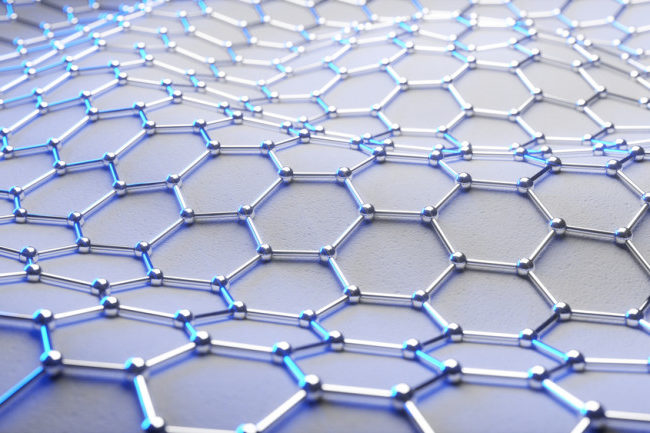
\includegraphics[width=5.2cm,height=3.8cm]{graficas/graphene.jpg}
		\justifying
			El grafeno (red bidimensional de átomos de carbono), catalogado como “el material del futuro”, ha sido objeto de estudio para la comunidad cient\'ifica debido a sus propiedades opto-electrónicas de gran inter\'es.\\
			\vspace{0.5cm}
			El presente trabajo de grado describe el comportamiento oscilatorio de la conductividad el\'ectrica como funci\'on de un campo magnético aplicado
			y su dependencia con la temperatura.
%			\end{multicols}
		\end{frame}

	\section{Planteamiento}
		\begin{frame}{Planteamiento y justificación del problema.}
			\justifying
			El grafeno exhibe propiedades que lo hacen muy interesante para la ciencia y para aplicaciones tecnológicas.\\
			Cada vez hay más dispositivos basados en grafeno y se hace necesario tener un mayor entendimiento teórico
			de las propiedades físicas de las estructuras basadas en grafeno.\\
			\vspace{0.5cm}
			En este contexto, el presente trabajo realiza una descripción teórica de la conductividad eléctrica
			en un sistema de una monocapa de grafeno colocada sobre un cristal de nitruro de Boro hexagonal (hBN).
		\end{frame}

		\begin{frame}{Planteamiento del problema}
			\justifying
			Con base en lo expuesto anteriormente, se plantea el siguente interrogante:
			\begin{itemize}
				\item ¿Cuál es la dependencia con la temperatura de las oscilaciones magnéticas de la conductividad eléctrica?
			\end{itemize}
		\end{frame}


	\section{Objetivos}
		\begin{frame}{Objetivo general}
			\justifying
			\begin{itemize}
    		\item Estudiar oscilaciones de la conductividad eléctrica en estructuras basadas en grafeno como función del campo magnético aplicado.
				\end{itemize}
		\end{frame}

		\begin{frame}{Objetivos específicos}
			\justifying
			\begin{enumerate}
			    \item Resolver la ecuación de Schrödinger para una estructura sustrato-grafeno en presencia de un campo magnético externo.
			    \item<2-> Determinar la densidad de estado del sistema.
			    \item<3-> Obtener la conductividad eléctrica del sistema.
			    \item<4-> Calcular la dependencia con respecto a la temperatura de las oscilaciones magnéticas en estructuras basadas en grafeno.
			\end{enumerate}

		\end{frame}

	\section{Metodología}
		\begin{frame}{Metodología}
			\justifying
			\begin{enumerate}
				\item Estudiar las propiedades y la f\'isica general del grafeno.
				\item<2-> A partir del Hamiltoniano del sistema, resolver la ecuaci\'on de Schrödinger.
				\item<3-> Hallar los niveles de Landau del espectro de energ\'ia.
				\item<4-> Determinar la funci\'on de Green asociada a los estados de banda del sistema.
				\item<5-> Determinar la densidad de estados del sistema.
				\item<6-> Estudiar el comportamiento oscilatorio de la conductividad el\'ectrica como funci\'on de la temperatura.
				\item<7-> Realizar c\'alculos num\'ericos.
			\end{enumerate}
		\end{frame}
